\documentclass{article}

\usepackage{tikz, amsmath, amssymb}
%\usepackage[margin=1.2in]{geometry}

\newcommand{\pder}[2]{\frac{\partial #1}{\partial #2}}
\title{Implementing Graph Convolution Network}

\author{
	Rajarshi Dasgupta
	}

\newcommand{\mat}[1]{\ensuremath{
	\begin{bmatrix}
		#1
	\end{bmatrix}
	}}
\newcommand{\gcnForPassTikz}[1]{
	\begin{center}
		\begin{tikzpicture}[scale = #1]
			%\draw  (-4,-2) node[below] {P} -- (4,-2) node[below] {Q} -- (4,2) node[above] {R} -- (-4,2) node[above] {S} -- (-4,-2);
			\draw (0,0) node[left] {$h^{(l)}_{w_1}$} -- (1,1);
			\draw (0,1) node[left] {$h^{(l)}_{w_2}$} -- (1,1);
			\draw (0,2) node[left] {$h^{(l)}_{w_3}$} -- (1,1);
			\draw[->] (1,1) -> (2,1) node[below] {mean};
			\draw[->] (2,1) -> (4,1) node[below] {$W^{(l)}$};
			\draw (4,1) -- (4.5,1);
			\draw[->] (5,-1) node[below] {$h^{(l)}_v$} -> (5,0) node[right] {$B^{(l)}$};
			\draw (5,0) -- (5,0.5);
			\node[circle, draw, radius=1] at (5,1) {$+$}; % Not nice
			\draw[->] (5.5,1) -> (6.5,1) node[below] {$\sigma^{(l)}$};
			\draw[->] (6.5,1) -> (7.5,1) node[right] {$h^{(l+1)}_v$};
		\end{tikzpicture}

		Layer $l$, node $v$, $N(v) = \{w_1, w_2, w_3\}$
	\end{center}
	}
\begin{document}

	\begin{itemize}
		\item Set of nodes $|V| = n$
		\item Set of edges $E \subseteq V \times V$
		\item Set neighbours of node $v$ is $N(v) = \{ u : (u,v) \in E \}$
		\item In-degree is $|N(v)|$
		\item Adjacency matrix $A$
			\begin{align*}
				a_{i,j} =
				\begin{cases}
					1 & \mbox{if } (i,j) \in E \\
					0 & \mbox{otherwise}
				\end{cases}
			\end{align*}
		\item Mesh consists of Vertices, Edges and Faces
		\item Graph Convolution Network (GCN) \\
			is a special case of Graph Neural Network (GNN)
	\end{itemize}

			\begin{center}
				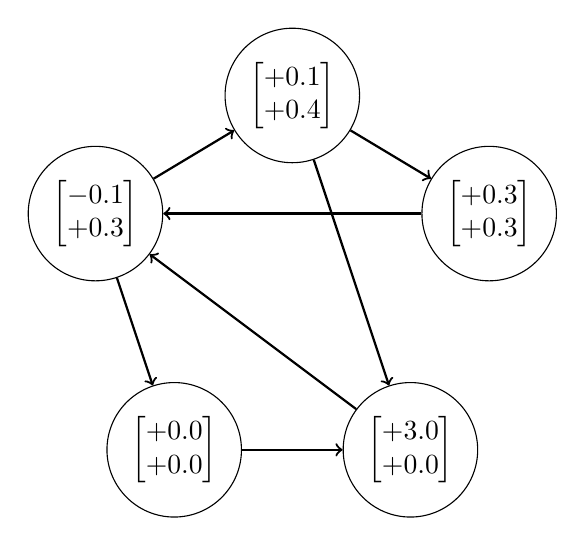
\begin{tikzpicture}
					\node (A) at (0,0)      [draw, circle] {\mat{+0.0 \\ +0.0}};
					\node (B) at (3,0)      [draw, circle] {\mat{+3.0 \\ +0.0}};
					\node (C) at (1.5,4.5)  [draw, circle] {\mat{+0.1 \\ +0.4}};
					\node (D) at (4,3)      [draw, circle] {\mat{+0.3 \\ +0.3}};
					\node (E) at (-1,3)     [draw, circle] {\mat{-0.1 \\ +0.3}};

					% Draw an arrow between the nodes
					\draw[->, thick] (A) -- (B);
					\draw[->, thick] (C) -- (B);
					\draw[->, thick] (D) -- (E);
					\draw[->, thick] (C) -- (D);
					\draw[->, thick] (E) -- (C);
					\draw[->, thick] (E) -- (A);
					\draw[->, thick] (B) -- (E);
				\end{tikzpicture}
			\end{center}

			\begin{itemize}
				\item Layer $l=0$
				\item $n_l = 2$
				\item $h_v^{(l)} \in \mathbb{R}^{n_l}$
			\end{itemize}

			\begin{center}
				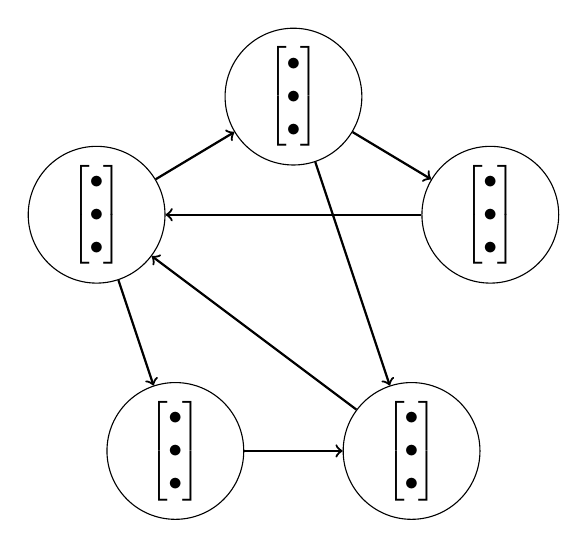
\begin{tikzpicture}
					\node (A) at (0,0)     [draw, circle] {\mat{\bullet \\ \bullet \\ \bullet}};
					\node (B) at (3,0)     [draw, circle] {\mat{\bullet \\ \bullet \\ \bullet}};
					\node (C) at (1.5,4.5) [draw, circle] {\mat{\bullet \\ \bullet \\ \bullet}};
					\node (D) at (4,3)     [draw, circle] {\mat{\bullet \\ \bullet \\ \bullet}};
					\node (E) at (-1,3)    [draw, circle] {\mat{\bullet \\ \bullet \\ \bullet}};

					% Draw an arrow between the nodes
					\draw[->, thick] (A) -- (B);
					\draw[->, thick] (C) -- (B);
					\draw[->, thick] (D) -- (E);
					\draw[->, thick] (C) -- (D);
					\draw[->, thick] (E) -- (C);
					\draw[->, thick] (E) -- (A);
					\draw[->, thick] (B) -- (E);
				\end{tikzpicture}
			\end{center}

			\begin{itemize}
				\item Layer $l=1$
				\item $n_l = 3$
				\item $h_v^{(l)} \in \mathbb{R}^{n_l}$
				\item Same graph
				\item Transformed node vectors
			\end{itemize}

	\gcnForPassTikz{0.75}

	\begin{itemize}
		\item $h_v^{(l)} \in \mathbb{R}^{n_l}$
		\item Each layer the node vector is transformed
		\item Layer $l$ has activation function $\sigma^{(l)}: \mathbb{R} \rightarrow \mathbb{R}$
		\item Trainable parameters
			$W^{(l)},B^{(l)} \in \mathbb{R}^{n_{(l+1)} \times n_l}$
		\item Forward pass
			$h_v^{(l+1)} = \sigma^{(l)}(W^{(l)} \sum_{w \in N(v)} \frac{h_w^{(l)}}{|N(v)|} + B^{(l)} h_v^{(l)})$ \\
			for $l = 0, 1, 2 \dots$
	\end{itemize}

	\begin{center}
		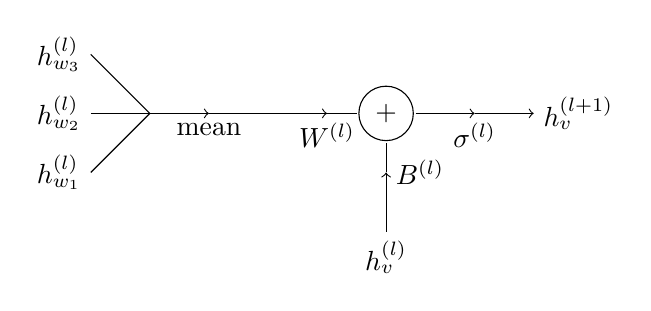
\begin{tikzpicture}[scale = 0.75]
			%\draw  (-4,-2) node[below] {P} -- (4,-2) node[below] {Q} -- (4,2) node[above] {R} -- (-4,2) node[above] {S} -- (-4,-2);
			\draw (0,0) node[left] {$h^{(l)}_{w_1}$} -- (1,1);
			\draw (0,1) node[left] {$h^{(l)}_{w_2}$} -- (1,1);
			\draw (0,2) node[left] {$h^{(l)}_{w_3}$} -- (1,1);
			\draw[->] (1,1) -> (2,1) node[below] {mean};
			\draw[->] (2,1) -> (4,1) node[below] {$W^{(l)}$};
			\draw (4,1) -- (4.5,1);
			\draw[->] (5,-1) node[below] {$h^{(l)}_v$} -> (5,0) node[right] {$B^{(l)}$};
			\draw (5,0) -- (5,0.5);
			\node[circle, draw, radius=1] at (5,1) {$+$}; % Not nice
			\draw[->] (5.5,1) -> (6.5,1) node[below] {$\sigma^{(l)}$};
			\draw[->] (6.5,1) -> (7.5,1) node[right] {$h^{(l+1)}_v$};
		\end{tikzpicture}
	\end{center}

	\vspace{-2em}

			\begin{figure}
			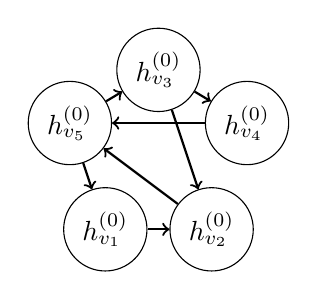
\begin{tikzpicture}[scale=0.45]
					\centering
					\node (A) at (0,0)     [draw, circle] {$h_{v_1}^{(0)}$};
					\node (B) at (3,0)     [draw, circle] {$h_{v_2}^{(0)}$};
					\node (C) at (1.5,4.5) [draw, circle] {$h_{v_3}^{(0)}$};
					\node (D) at (4,3)     [draw, circle] {$h_{v_4}^{(0)}$};
					\node (E) at (-1,3)    [draw, circle] {$h_{v_5}^{(0)}$};
					% Draw an arrow between the nodes
					\draw[->, thick] (A) -- (B);
					\draw[->, thick] (C) -- (B);
					\draw[->, thick] (D) -- (E);
					\draw[->, thick] (C) -- (D);
					\draw[->, thick] (E) -- (C);
					\draw[->, thick] (E) -- (A);
					\draw[->, thick] (B) -- (E);
			\end{tikzpicture}
			\end{figure}

			\begin{align*}
				\rightarrow
			\end{align*}

			\begin{figure}
			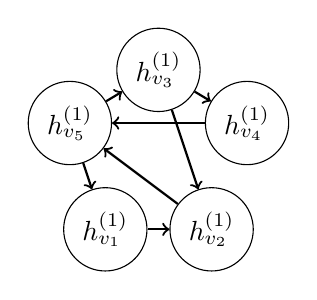
\begin{tikzpicture}[scale=0.45]
					\centering
					\node (A) at (0,0)     [draw, circle] {$h_{v_1}^{(1)}$};
					\node (B) at (3,0)     [draw, circle] {$h_{v_2}^{(1)}$};
					\node (C) at (1.5,4.5) [draw, circle] {$h_{v_3}^{(1)}$};
					\node (D) at (4,3)     [draw, circle] {$h_{v_4}^{(1)}$};
					\node (E) at (-1,3)    [draw, circle] {$h_{v_5}^{(1)}$};
					% Draw an arrow between the nodes
					\draw[->, thick] (A) -- (B);
					\draw[->, thick] (C) -- (B);
					\draw[->, thick] (D) -- (E);
					\draw[->, thick] (C) -- (D);
					\draw[->, thick] (E) -- (C);
					\draw[->, thick] (E) -- (A);
					\draw[->, thick] (B) -- (E);
				\end{tikzpicture}
			\end{figure}

			\begin{center}
				Layer 0
			\end{center}
			\begin{center}
				Layer 1
			\end{center}

	We can rewrite the forward-pass relation in the following manner
	\begin{align*}
		h_v^{(l+1)} &= \sigma^{(l)} ( W^{(l)} \sum_{w \in N(v)} \frac{h_w^{(l)}}{|N(v)|} + B^{(l)} h_v^{l}) \\
		\implies H^{(l+1)} &= \sigma^{(l)}( D^{-1} A H^{(l)} W^{(l)\mathsf{T}} + H^{(l)} B^{(l)\mathsf{T}} )
	\end{align*}

	Where,
	\begin{align*}
		H^{(l)} =
		\begin{bmatrix}
			h_1^{(l)\mathsf{T}} \\
			\vdots \\
			h_n^{(l)\mathsf{T}}
		\end{bmatrix} \,&
		D = 
		\begin{bmatrix}
			d_1 & & \\
			& \ddots & \\
			& & d_n
		\end{bmatrix} \\
		d_v &= |N(v)|
	\end{align*}

	This is more suitable for implementation purposes \\
	as matrix vector operations are highly optimised

\end{document}


